\chapter{Syntax trees}

\epigraph{in the forest:\\
some trees reach up\\
some trees reach out\\
all trees reach}{}

\section{Introduction}

In previous chapters, we've explored the building blocks of English grammar: words, phrases, and their functions. Now, we'll introduce a useful tool for visualizing how these elements come together to form sentences: syntax trees.

\begin{wrapfigure}{r}{0.5\textwidth} % "r" for right alignment, "0.5\textwidth" for width of the figure
  \centering
  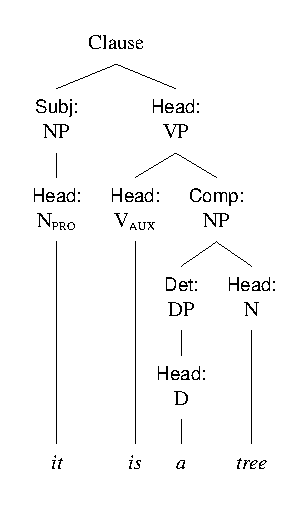
\includegraphics[width=0.8\textwidth]{figures/itisatree.pdf}
  \caption{A \textsc{syntax tree}}
  \label{fig:tree1}
\end{wrapfigure}

Syntax trees are diagrams that represent the hierarchical structure of sentences, showing how words combine into phrases, and phrases into larger units. While you likely won't use these diagrams directly in your ESL classroom, understanding them will deepen your grasp of English syntax and sharpen your ability to analyze language structures.


This chapter guides you through the basic principles of syntax trees. It will show you how to read and construct these diagrams, along with ways that trees can clarify ambiguous sentences. And it will lay out the pedagogical value of syntax trees for language teachers.

By the end of this chapter, you'll have a new perspective on sentence structure~-- one that will enhance your understanding of English grammar and, in turn, your effectiveness as an ESL teacher. Let's begin by exploring what these trees look like and why they're useful.




% the commands such as \Head don't seem to be working, so I'll include a PDF
%\begin{forest}
%where n children=0{% for each terminal node
%    font=\itshape, 			% italics
%    tier=word          			% align at the "word" tier (bottom)
%  }{%								% no false conditions, so empty
%  },
%[Clause
%	[Section ubj{NP}[\Head{N\textsubscript{\textsc{pro}}}[it]]]
%	[\Head{VP}
%		[\Head{V\textsubscript{\textsc{aux}}}[is]]
%		[\Comp{NP}
%			[\Det{DP}[\Head{D}[a]]]
%			[\Head{N}[tree]]
%		]
%	]
%]
%\end{forest}

\section{A first tree}

Figure \ref{fig:tree1} is a \textsc{syntax tree}. Starting at the bottom right, it tells you that there is a word \textit{tree}. Follow that branch up and you'll see Head:N, which means that this is a noun functioning as the head of something. If you follow that next branch up, you can see that it's the head of a noun phrase (NP). Back down at the bottom, the second last word is \textit{a}, which is labeled Head:D. D is short for determinative (the category). Following its branch upwards, we see it's the head of a determinative phrase (DP). This determinative phrase functions as the determiner (Det) for the NP with the head noun \textit{tree}.

Moving to the left, we encounter the verb \textit{is}, labeled as a verb with the subscript \textsc{aux}, indicating its special categorization as an auxiliary verb (one of the small group that has the NICER properties; see Section \ref{sec:aux}). This verb functions as the head of the verb phrase (VP). The VP also contains a complement (Comp), which is the noun phrase we discussed earlier (with the head noun \textit{tree}).

Further to the left, we have the pronoun \textit{it}. This word is labeled as a noun with the subscript \textsc{pro}, indicating it's a pronoun. Following its branch up, we find it's labeled as the head of an NP, and this NP functions as the subject (Subj) of the clause.

The entire structure is labeled as a clause, which is the highest level of this tree. This clause contains both a subject (the NP with the pronoun \textit{it}) and a predicate (the VP with the auxiliary verb \textit{is} and its complement).

\section{Syntax trees, a solar-system metaphor}\label{sec:trees}

Consider the solar system as a metaphor to understand categories and functions in language, particularly the functions of \textit{head} and \textit{dependent}. In the solar system, the central entity is the Sun, which serves as the ``head'' of the system. Everything else, from planets to dust, depends on the Sun, making them ``dependents.'' We can draw this as the tree in Figure \ref{fig:solarsys}.

\begin{figure}
  \centering
  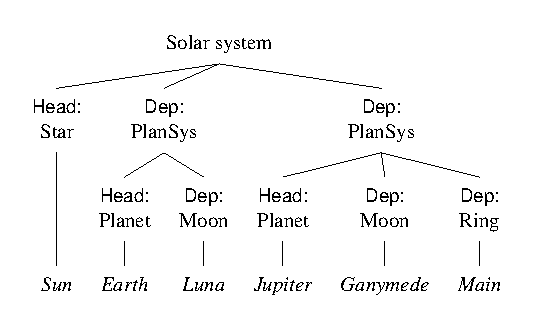
\includegraphics{figures/solarsys.pdf}
  \caption{A partial tree of the solar system}
  \label{fig:solarsys}
\end{figure}

Consider the categories and functions in the solar system:
\begin{itemize}[noitemsep]
    \item The Sun belongs to the \textsc{star} category. This star functions as the head of the \textsc{solar system}.
    \item Jupiter, Earth, Venus, etc. belong to the \textsc{planet} category. Each of these planets functions as the head of a \textsc{planetary system} (PlanSys), and those planetary systems are dependents (Dep) in the solar system.
    \item Within each planetary system:
    \begin{itemize}[noitemsep]
        \item The planet itself, such as Earth or Jupiter, is the head.
        \item Satellites around the planets are categorized as \textsc{Moon} or \textsc{Ring}. These function as dependents in their respective planetary systems.
    \end{itemize}
\end{itemize}


\begin{wrapfigure}{r}{0.5\textwidth} % "r" for right alignment, "0.5\textwidth" for width of the figure
  \centering
  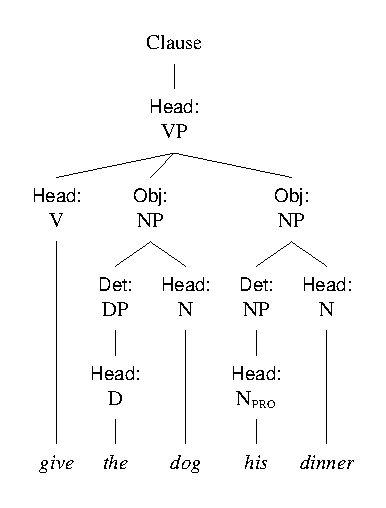
\includegraphics[width=0.8\textwidth]{figures/dogdinner.pdf}
  \caption{Another syntax tree}
  \label{fig:tree2}
\end{wrapfigure}

This hierarchical structure of heads and dependents isn't limited to the solar system. For instance, our solar system is a dependent within the larger \textsc{galaxy}, which has its own head: a \textsc{supermassive black hole}.

Applying this metaphor to language, consider a verb phrase. Just as the Sun is the head of the solar system, the verb (e.g., \textit{give}) is the head of a verb phrase. Without the verb \textit{give}, the connection between \textit{the dog} and \textit{his dinner} is lost. Both \textit{the dog} and \textit{his dinner} are dependents in the VP. Specifically, they are objects, a sub-type of complement, which, in turn, is a kind of dependent. The tree is shown in Figure \ref{fig:tree2}.


Breaking it down further:
\begin{itemize}[noitemsep]
    \item \textit{Give} is the head of the VP.
    \item \textit{The dog} is an NP functioning as an object. 
    \item Within this NP, the noun \textit{dog} is the head, and the determinative \textit{the} is the determiner.
    \item \textit{His dinner} is another noun phrase object. Here, the noun \textit{dinner} is the head, and the pronoun \textit{his} is the determiner.
\end{itemize}

This structure showcases how different phrases in language have heads and dependents, similar to the entities in our solar system.

\section{Why syntax trees?} \label{sec:why-trees}

Syntax trees are visual models of the relations between words and phrases in larger constructions. They are common in linguistics, but they are rarely used in language teaching. To be clear, I'm not employing trees in this book so that you can use them in your teaching. While a particularly academically oriented student may find trees useful in understanding the structure of sentences, the level of detail involved is generally not a level that students need.

So, why employ trees?

\begin{enumerate}[noitemsep]
    \item \textbf{Better learning through dual-encoding:} As I said, syntax trees provide a visual representation of the relations between words and phrases in larger constructions. There is good evidence that multi-modal learning is more effective than learning that takes place in a single modality \citep{ginns2005}. And so, it's likely that by employing syntax trees alongside other methods, you will be able to recall the ideas of phrase structures, categories, and functions.
    \item \textbf{Brevity and clarity:} As you can see above, it takes a paragraph or more to describe the information set out in a simple syntax tree, and the explanation is often much harder to understand.
    \item \textbf{Explicitness:} When you draw a tree, you take an explicit position on the categories of words and phrases, along with their functional relationships. This is much more difficult in prose, which means that prose descriptions tend to be vague. As a result, it's much easier in prose to fool yourself into thinking that you've understood when you haven't. With trees, it is obvious when the analysis is correct.
    \item \textbf{Practice with explicit feedback:} There is very strong evidence that mastery is achieved through deliberate practice \citep{ericsson1993}. Deliberate learning will be addressed in some depth in the vocabulary module (Section \ref{sec:delib}), but, simply put, it involves the following cycle: attempt $\rightarrow$ explicit feedback $\rightarrow$ reflection $\rightarrow$ attempt. Employing trees allows you to easily get quick, accurate feedback by comparing trees you draw to the answer key.
\end{enumerate}

\noindent In short, we are employing trees because they are an extremely effective tool for learning syntax and for demonstrating that learning.

\section{Composing your trees}

\subsection{Marking specific dependents}\label{sec:MardDeps}

\begin{wrapfigure}{r}{0.5\textwidth} % "r" for right alignment, "0.5\textwidth" for width of the figure
  \centering
  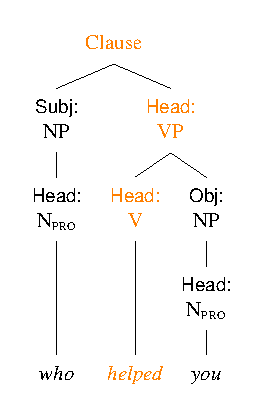
\includegraphics[width=0.8\textwidth]{figures/whohelpedyou.pdf}
  \caption{Tree for \textit{Who helped you?}}
  \label{fig:tree3}
\end{wrapfigure}

The tree diagram presented in Figure \ref{fig:tree3} can be interpreted as a single tree or as a combination of three smaller trees, distinguishable by their colors: one black, one orange, and another black.

Starting at the bottom of the rightmost black tree, there's the word \textit{you}. \textit{You} a pronoun, is a specific type of noun, so it's labeled with an N. This pronoun, \textit{you}, functions as the head of an NP.

Jumping to the leftmost black tree, \textit{who} is another pronoun and is similarly labeled. It functions as the head of its NP.

The orange tree is centered around the word \textit{helped}, a verb. Its verb status is evident from its past-tense form, a feature exclusive to verbs. This verb is the head of a VP, analogous to how the noun is the head of an NP. The VP, in turn, is the head of the whole clause.

Each of the NPs functions as a dependent; the \textit{who} NP is a dependent in the clause, while the \textit{you} NP is a dependent in the VP. But we can consult Section \ref{sec:Dep} to see more precisely what kind of dependent each is. \textit{You} is an NP in a VP, and it's you who is being helped, which is to say, being acted upon. And if we make the sentence passive (\textit{you were helped}), \textit{you} becomes the subject. All of which is to say, it has all the characteristics of an object.

We can go through the same process with \textit{who}. It's an NP at the start of a clause, and it denotes the person doing the helping. It's not really the topic, and we can't check agreement because the verb is not present tense, but it seems like \textit{who} must be the subject.

To ensure the accuracy of tree diagram, I'll apply the checks from Section \ref{sec:checkTrees}. The topmost label should be a phrasal category like \textit{Clause}, \textit{NP}, or \textit{VP} without any function \ding{51}. Each branch should culminate in a single word at its base \ding{51}. As we trace up a branch, we should encounter a label indicating \textit{head X}, where X is a lexical category \ding{51}. Continuing upwards, the next label should indicate a function and then a phrasal category \ding{51}. This pattern should persist until reaching the topmost label.

\paragraph*{A note on tree styles}

Linguists have many different ways to draw syntax trees. You can find trees of the style I present here in \textit{CGEL} or in \textit{A student's introduction to English grammar} \citep{huddleston2022}. If you want to search online for more examples, be sure to include \textit{CGEL} in your search query. Otherwise, you could end up with something rather different.

\subsection{A top-down example}

Let's try creating a syntax tree for the clause \textit{I had my breakfast}. We'll start at the top and work down and left to right. So, since this is a clause, we put that at the top:
\par
{
\centering
Clause
\par
}

Now, let work left to right. \textit{I} is a subject NP, so we add a branch sloping down and to the left from the Clause label. The function goes above the category, so Subj: on the first line and NP below it.

\begin{figure}[H]
    \centering
    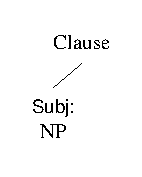
\includegraphics{figures/ihadmybreakfast.pdf}
    \label{fig:breakfast1}
\end{figure}

This NP needs a head, so we add a branch going straight down and label it Head:N\textsubscript{\textsc{pro}}.

\begin{figure}[H]
    \centering
    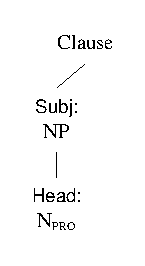
\includegraphics{figures/ihadmybreakfast2.pdf}
    \label{fig:breakfast2}
\end{figure}

And finally, we add \textit{I}.

\begin{figure}[H]
    \centering
    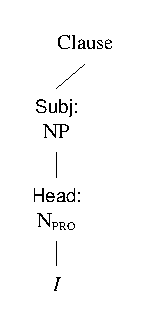
\includegraphics{figures/ihadmybreakfast3.pdf}
    \label{fig:breakfast3}
\end{figure}

Next, we'll add the Head:VP on a rightwards sloping branch from the Clause.

\begin{figure}[H]
    \centering
    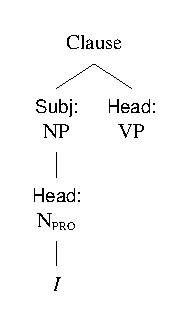
\includegraphics{figures/ihadmybreakfast4.pdf}
    \label{fig:breakfast4}
\end{figure}

This VP has a head:V, and terminates in \textit{helped}. There's also \textit{you}, so, the branch from the VP should slope leftwards.

\begin{figure}[H]
    \centering
    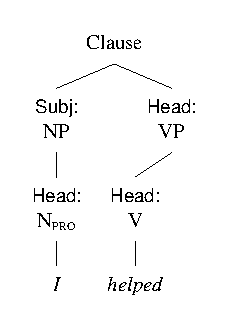
\includegraphics{figures/ihadmybreakfast5.pdf}
    \label{fig:breakfast5}
\end{figure}

Finally, we'll add the object:NP, with its head:N\textsubscript{\textsc{pro}} and its terminal \textit{you}.

\begin{figure}[H]
    \centering
    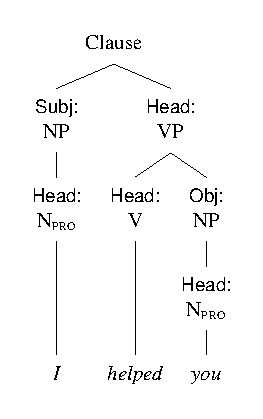
\includegraphics{figures/ihadmybreakfast6.pdf}
    \label{fig:breakfast6}
\end{figure}

Some people prefer to start with the sentence at the bottom of the page and work up through the lexical category head, the phrasal category and its function, etc. Play with both ways and see what works for you.





\subsection{Some trees}

Let's start with a very simple tree (\ref{tree:happy}). We'll start with a single-branching AdjP composed only of a Head.
\begin{itemize}[noitemsep]
    \item As always, the top node is a phrasal category, in this case AdjP. There's no function because functions are relational, and this AdjP is not in a relation.
    \item The very bottom of our tree is a word node, in this case \textit{happy}.
    \item Immediately above \textit{happy} is a node with a function labeled Head. This is the function of \textit{happy} in the AdjP. It also has the category label Adj, which tells us that \textit{happy} is an adjective.
\end{itemize}

\ea \raisebox{-0.8\height}{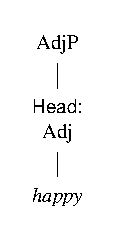
\includegraphics{figures/happy.pdf}}\label{tree:happy}
\z


Let's try another one (\ref{tree:very}). This time we have a single-branching AdvP.
\begin{itemize}[noitemsep]
    \item As always, the top node is a phrasal category, in this case AdvP. There's no function because functions are relational, and this AdvP is not in a relation.
    \item The very bottom of our tree is a word node, in this case \textit{very}.
    \item Immediately above \textit{very} is a node with a function labeled Head. This is the function of \textit{very} in the AdvP. It also has the category label Adv, which tells us that \textit{very} is an adverb.
\end{itemize}

\ea \raisebox{-0.8\height}{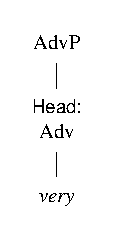
\includegraphics{figures/very.pdf}}\label{tree:very}
\z



Let's put these together in (\ref{tree:veryhappy}). This time we have a double-branching AdjP.
\begin{itemize}[noitemsep]
    \item As always, the top node is a phrasal category, in this case AdjP. There's no function because functions are relational, and this AdjP is not in a relation.
    \item If you start at the top and follow the right-hand branch, you see we have simply reproduced the AdjP from (\ref{tree:happy}).
    \item On the left, though, we have the AdvP from (\ref{tree:very}), but this time it's in a relation in the AdjP, so it has a function. Its function in the AdjP is Modifier.
\end{itemize}

\ea \raisebox{-0.8\height}{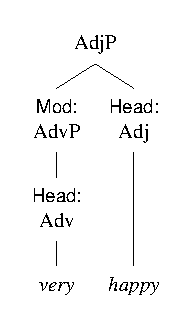
\includegraphics{figures/veryhappy.pdf}}\label{tree:veryhappy}
\z

This is the basis of all trees. Below the picture, we'll repeat this with the PP \textit{about it}. Before scrolling down, try drawing trees like (\ref{tree:happy}--\ref{tree:veryhappy}) for \textit{about}, \textit{it}, and \textit{about it}.

We'll try that again in (\ref{tree:about}). We start with a single-branching PP.
\begin{itemize}[noitemsep]
    \item As always, the top node is a phrasal category, in this case PP. There's no function because functions are relational, and this PP is not in a relation.
    \item The very bottom of our tree is a word node, in this case \textit{about}.
    \item Immediately above \textit{about} is a node with a function labeled Head. This is the function of \textit{about} in the PP. It also has the category label P, which tells us that \textit{about} is a preposition.
\end{itemize}

\ea \raisebox{-0.8\height}{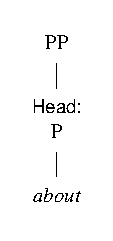
\includegraphics{figures/about.pdf}}\label{tree:about}
\z

This time we have a single-branching NP (\ref{tree:it}). Remember that pronouns are a special kind of noun.
\begin{itemize}[noitemsep]
    \item As always, the top node is a phrasal category, in this case NP. There's no function because functions are relational, and this NP is not in a relation.
    \item The very bottom of our tree is a word node, in this case \textit{it}.
    \item Immediately above \textit{it} is a node with a function labeled Head. This is the function of \textit{it} in the NP. It also has the category label N, which tells us that \textit{it} is a noun (specifically a pronoun).
\end{itemize}

\ea \raisebox{-0.8\height}{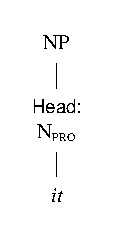
\includegraphics{figures/it.pdf}}\label{tree:it}
\z

This time we have a double-branching PP.
\begin{itemize}[noitemsep]
    \item As always, the top node in \ref{tree:aboutit} is a phrasal category, in this case PP. There's no function because functions are relational, and this PP is not in a relation.
    \item If you start at the top and follow the left-hand branch, you see we have simply reproduced the PP from (\ref{tree:about}). Note that in (\ref{tree:veryhappy}) the Head was on the right and here it's on the left. There's no rule about which side the Head goes on. It depends on which dependents we find.
    \item On the right, though, we have the NP from (\ref{tree:it}), but this time it's in a relation in the PP, so it has a function. Its function in the PP is Complement. (More specifically, it is an object.)
\end{itemize}

\ea \raisebox{-0.8\height}{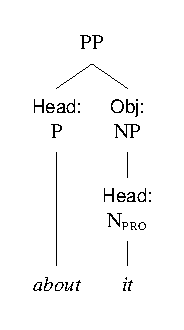
\includegraphics{figures/aboutit.pdf}}\label{tree:aboutit}
\z

Now we'll try putting (\ref{tree:veryhappy}) and (\ref{tree:aboutit}) together in the AdjP \textit{very happy about it} (\ref{tree:veryhappyaboutit}). Try drawing this before scrolling down to check. Here's our final tree, the AdjP \textit{very happy about it}.
\begin{itemize}[noitemsep]
    \item As always, the top node is a phrasal category, in this case AdjP. There's no function because functions are relational, and this AdjP is not in a relation.
    \item If you start at the top and follow the middle branch, you see we have simply reproduced the AdjP from (\ref{tree:happy}), and the leftmost two branches are just the AdjP from (\ref{tree:veryhappy}).
    \item The right-hand branch is the PP from (\ref{tree:aboutit}). But this time it's in a relation in the AdjP, so it has a function. Its function in the AdjP is Complement.
    \item Notice that there is a complement inside a complement. This property of being able to put one thing inside a thing of the same kind is called \textsc{recursion} (or ``nesting'').
\end{itemize}

\ea \raisebox{-0.8\height}{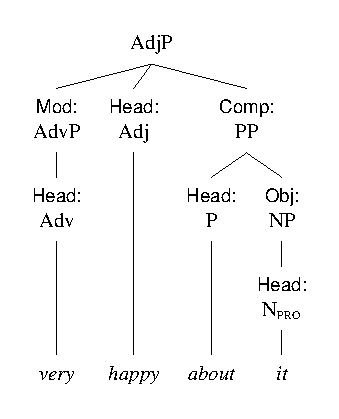
\includegraphics{figures/veryhappyaboutit.pdf}}\label{tree:veryhappyaboutit}
\z

\subsection{Identifying constituents}\label{sec:identifying_constituents}

When drawing more complex syntax trees, it can be challenging to identify the \textbf{constituents} of your sentence. Constituents are groups of words that function as a single unit within the phrase structure. Determining what constitutes a constituent is crucial because it informs how you will structure your tree.

To identify constituents, you can use several \textbf{constituency tests}. Here are the four primary tests you can apply:

\begin{enumerate}[noitemsep]
    \item \textbf{Coordination Test}
    \begin{itemize}[noitemsep]
        \item \textbf{Explanation}: If a group of words can be coordinated (joined with a conjunction like \textit{and} or \textit{or}) with a similar group, it's likely a constituent.
        \item \textbf{Example}:
        \begin{itemize}[noitemsep]
            \item Original: \textit{My well-meaning aunt gave all her loyalty cards \underline{to the kind man who helped you}.}
            \item Coordination: \textit{My well-meaning aunt gave all her loyalty cards \underline{to the kind man who helped you} and \underline{to the woman at the counter}.}
        \end{itemize}
        \item \textbf{Analysis}: The ability to coordinate \textit{to the kind man who helped you} with \textit{to the woman at the counter} suggests that it's a constituent.
    \end{itemize}
    
    \item \textbf{Proform Replacement Test}
    \begin{itemize}[noitemsep]
        \item \textbf{Explanation}: If a group of words can be replaced by a single proform (like \textit{he}, \textit{it}, \textit{there}), or \textit{do so}, it's likely a constituent.
        \item \textbf{Example}:
        \begin{itemize}[noitemsep]
            \item Original: \textit{My well-meaning aunt gave \underline{all her loyalty cards} to the kind man who helped you.}
            \item Replacement: \textit{My well-meaning aunt gave \underline{them} to the kind man who helped you.}
        \end{itemize}
        \item \textbf{Analysis}: Replacing \textit{all her loyalty cards} with \textit{them} indicates that it's a constituent.
    \end{itemize}
    
    \item \textbf{Ellipsis Test}
    \begin{itemize}[noitemsep]
        \item \textbf{Explanation}: If a group of words can be omitted without making the sentence ungrammatical (and the meaning remains clear), it's likely a constituent.
        \item \textbf{Example}:
        \begin{itemize}[noitemsep]
            \item Original: \textit{My well-meaning aunt gave all her loyalty cards to the kind man who helped you, and her friend did too.}
            \item Ellipsis: The omitted portion corresponds to \textit{gave all her loyalty cards to the kind man who helped you}.
        \end{itemize}
        \item \textbf{Analysis}: The omission of the repeated phrase suggests that it functions as a constituent.
    \end{itemize}
    
    \item \textbf{Dislocation (Preposing) Test}
    \begin{itemize}[noitemsep]
        \item \textbf{Explanation}: If a group of words can be moved to the beginning of a sentence without rendering it ungrammatical, it's likely a constituent.
        \item \textbf{Example}:
        \begin{itemize}[noitemsep]
            \item Original: \textit{My well-meaning aunt gave all her loyalty cards \underline{to the kind man who helped you}.}
            \item Dislocation: \textit{\underline{To the kind man who helped you}, my well-meaning aunt gave all her loyalty cards.}
        \end{itemize}
        \item \textbf{Analysis}: Moving \textit{to the kind man who helped you} to the front of the sentence suggests it's a constituent.
    \end{itemize}
\end{enumerate}

By applying these tests, you can determine how to break down the sentence into its constituent parts before drawing your syntax tree.


\subsection{Checking your trees}\label{sec:checkTrees}

After you draw a tree, you should complete the following seven checks.

\begin{enumerate}[noitemsep]
    \item The very top label is a phrasal category (e.g., Clause, VP, NP, etc.) with no function.
    \item No matter how many branches go down from that label, one and only one is labeled Head.
    \item At the very bottom of each branch, there is a single word (e.g., \textit{jump}, \textit{ball}, \textit{the}, etc.).
    \item If you trace that branch up from that word, you run into a label that says Head:X.
    \item That X is a lexical category (e.g., N, V, Adj, D, etc.), not a phrasal category.
    \item If you follow that branch up, the next label is \textsc{Function}:XP (e.g., Subj:NP, Mod:AdvP, Head:VP, etc.).
    \item This is true all the way up until the very top label, which doesn't include a function (see 1.).
\end{enumerate}

Try these checks on Figures \ref{fig:tree1} and \ref{fig:tree2}. It's possible, though unlikely, that I introduced an error there.

\section{More trees}\label{sec:more trees}

We'll now try some slightly more complex trees, using \textit{very happy about it}. First, we'll look at a simple clause: \textit{We won} (\ref{tree:wewon}).
\begin{itemize}[noitemsep]
    \item At the top, as always, we have a phrasal category label, in this case, Clause. Despite not calling it a ``Clause Phrase'', it is still a phrasal unit, consisting of a Head and any dependents.
    \item The Head of the clause is the VP, which, in turn, has the verb \textit{won} as its Head.
    \item The dependent in the Clause is the Subject, on the left. It's an NP headed by the (pro)noun \textit{we}.
\end{itemize}

\ea \raisebox{-0.8\height}{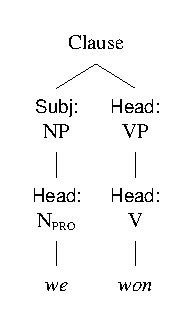
\includegraphics{figures/wewon.pdf}}\label{tree:wewon}
\z

Next, we will change \textit{won} to the auxiliary verb \textit{are}, and add the complement \textit{very happy about it}.
\begin{itemize}[noitemsep]
    \item This tree takes the basic form of (\ref{tree:happy}). The verb has changed from \textit{won} to \textit{are}, and we have added a complement.
    \item The complement is simply the AdjP from the previous section \textit{very happy about it}. The only difference is that there it wasn't in a relation, so it had no function label. Now it is the Complement of the VP, and its label reflects that.
\end{itemize}

\ea \raisebox{-0.8\height}{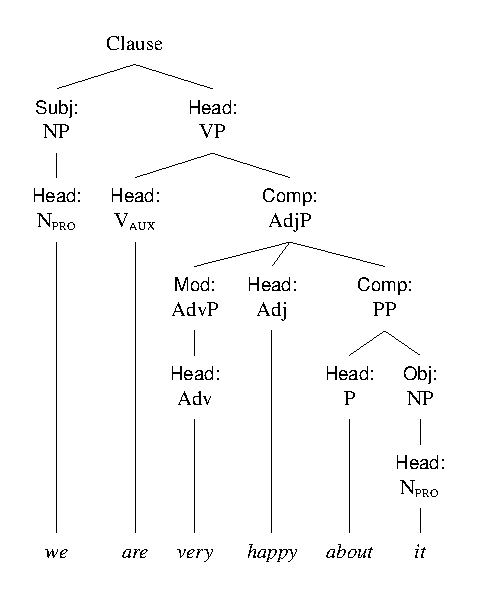
\includegraphics{figures/weareveryhappyaboutit.pdf}}\label{tree:weareveryhappyaboutit}
\z

Sometimes, linguists will use a triangle (or a ``coat hanger'') when they don't want to show the internal detail, usually because they don't have room on the page or because they want to focus on something else in the tree. We could, for example, replace the AdjP tree from (\ref{tree:weareveryhappyaboutit}) with a triangle, as in (\ref{tree:weareveryhappyaboutit2}).

\ea \raisebox{-0.8\height}{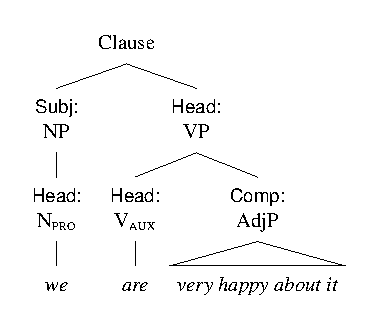
\includegraphics{figures/weareveryhappyaboutit2.pdf}}\label{tree:weareveryhappyaboutit2}
\z

\section{Disambiguating with trees}

A clause can be ambiguous, but a tree will usually disambiguate it by showing the structure. Consider \textit{Sherlock saw the man with the binoculars} in Figure \ref{fig:binoculars}. Out of context, this is ambiguous between a sighting via the binoculars or that of a man equipped with the binoculars.

\begin{figure}[h]
    \centering
    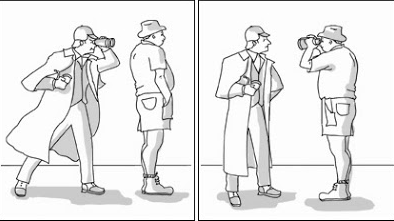
\includegraphics[width=0.8\textwidth]{figures/binoculars.png}
    \caption{Sherlock using binoculars to look at a man and Sherlock looking at a man who has binoculars}
    \label{fig:binoculars}
\end{figure}

We can show the two meanings with trees. In (\ref{tree:binoculars1}), the PP \textit{with the binoculars} is a modifier in the VP; it explains how the seeing was accomplished. In (\ref{tree:binoculars2}), the PP \textit{with the binoculars} is a modifier in the NP; it tells us about the man.

\ea
    \ea \raisebox{-0.8\height}{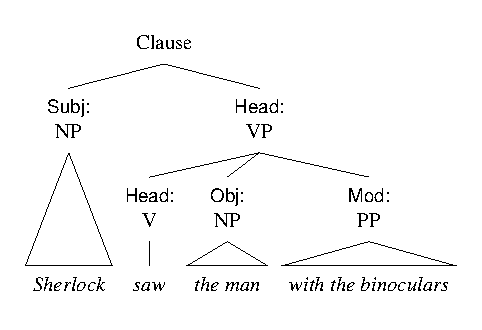
\includegraphics{figures/binoculars1.pdf}} \label{tree:binoculars1}
    \ex \raisebox{-0.8\height}{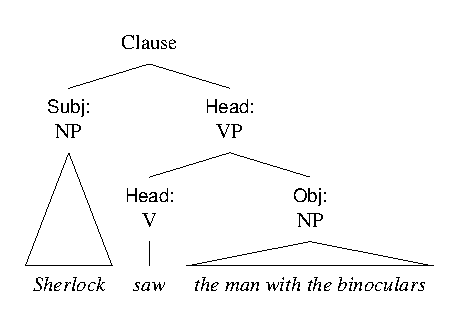
\includegraphics{figures/binoculars2.pdf}} \label{tree:binoculars2}
    \z
\z

\section{Do we need the function labels?}

Many linguists label only the categories, not the functions. This certainly produces less cluttered trees, but for language teachers, it's useful to be able to state the function of each constituent. It's also less clear if we omit the functions. Consider the difference between \textit{Brett and Michael, try harder} and \textit{Brett and Michael try harder}. The first one is an instruction to Brett and Michael, who have, it seems, been slacking off. The second is a positive statement about Brett and Michael's work ethic. If you avoid the function labels, the two sentences would have the same tree (\ref{tree:b+mtryharder}).

\ea\raisebox{-0.8\height}{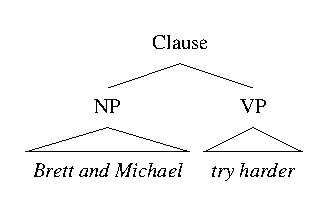
\includegraphics{figures/b+mtryharder.pdf}} \label{tree:b+mtryharder}
\z

But when we add function labels, we can identify whether Brett and Michael is a subject (\textit{Brett and Michael try harder} \ref{tree:b+mtryharder1}) or an adjunct (\textit{Brett and Michael, try harder} \ref{tree:b+mtryharder2}).\footnote{Adjunct is a function we haven't talked about yet, but it means roughly something that is stuck on. In this case it's calling out to Brett and Michael, like saying ``hey''.}

\ea
    \ea\raisebox{-0.8\height}{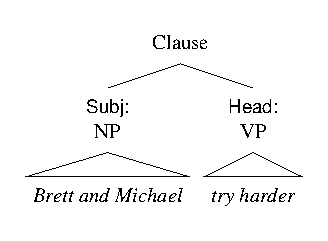
\includegraphics{figures/b+mtryharder1.pdf}} \label{tree:b+mtryharder1}
    \ex\raisebox{-0.8\height}{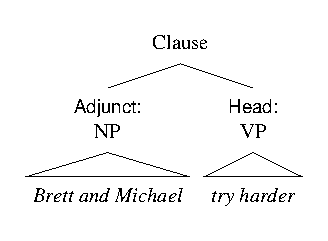
\includegraphics{figures/b+mtryharder2.pdf}} \label{tree:b+mtryharder2}
    \z
\z

\section{Some terminological issues} \label{sec:terminology}

You will often see expressions like ``adverbial'', ``adverb phrase'', or ``adverb clause'' used when there isn't a single adverb to be found. This is based on an entirely semantic idea of what it means to be ``adverbial''. Specifically, if something answers the questions ``when'', ``where'', ``why'', or ``how'', then many grammarians use the term \textsc{adverbial}.

They're not wrong.

Terminology is arbitrary. There's no inherently correct term. We could use a different term for what we're calling \textsc{determiners}. We could call them \textsc{specifiers} instead. Or we could call them \textsc{articles} or \textsc{markers} or \textsc{spoons} or \textsc{category 6}. In principle, any label should do.

We could even call them \textsc{Steve}.\footnote{\href{https://www.youtube.com/embed/CiGFRLCC-Ao}{Let's call it ``Steve''.}}

BUT.

While the label does not matter, the way we constitute the category does. And a category of things that ``answer the question `when', `where', `why', or `how''', based entirely on semantics, is not a useful syntactic category. By this definition, \textit{my birthday} is ``adverbial''. So is \textit{Toronto}, \textit{reasons}, and \textit{with binoculars}. But these things just don't go together. They don't make a coherent set, and you can't teach anybody anything useful about grammar by lumping them together.

Terms are just labels, and any label will work in principle.\footnote{In practice, if you use a highly eccentric label, obviously you will not be understood by many people. Recall the discussion of standards in Section \ref{sec:standards}.} But categories matter. They tell us about the world. And trying to make sense of badly constructed categories just makes life harder for everyone.

\section{Summary}
The main value of drawing syntax trees is to ensure you have a clear understanding of what each of the elements in sentence or phrase is and how they interrelate. You probably won't be showing syntax trees to students who are learning English, but they are useful tools for teachers who want to have a clear understanding of how English works.

At this point, we've only touched on a subset of the lexical and phrasal categories in very simple constructions. There is more to learn. In later chapters, we will look at coordination, subordination, and interrogatives. In the meantime, you should practice drawing very simple trees until you feel comfortable with them.

For now, we will shift focus to the English sound system.